\scanpage{146}
pour $i\neq n$, et (comme $x$ arbitraire) $u_i=0$ pour $i\neq n$.
Donc les \deleted{\unsure{hom|homs}}\inserted{morphismes} homogènes de degré 1 de $V(N)$ dans $V(M)$ correspondent exactement aux homs des $k$-modules
\[
M\mathbin{\text{---}}N
\]
(et sont par suite néc. $O_k$-linéaires !). Cela prouve en $=$ temps la pleine fidélité.

On détermine de $=$ les morphismes
\[
\prod_{i\in I}V(N_i)\longrightarrow\deleted{\unsure{V}}F
\]
\[
\deleted{\unsure{\wr}\quad V\left(\coprod_iN_i\right)}
\]
Compte tenu de l'isom évident
\[
\prod_{\alpha\in I}V(N_\alpha)\simeq V\left(\bigoplus N_\alpha\right)
\]
\margin{\figure{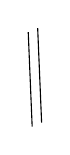
\begin{tikzpicture}\draw (0,0)--(0.05,-1.2);\draw (0.12,0.05)--(0.17,-1.15);\end{tikzpicture}}}
(de façon générale il est trivial que $V$ transforme $\unsure{\varinjlim}$ quelc. en $\varprojlim$).
Dans le cas de $F=V(M)$, ceci correspond donc aux hom
\[
M\xrightarrow{u}\operatorname{Sym}^*\left(\bigoplus N_\alpha\right)
=\bigotimes_\alpha\operatorname{Sym}^*(N_\alpha)
\]
Ici il y a lieu de décomposer $M$ suivant les multidegr. $i=(i_\alpha)_{\alpha\in I}\in\mathbb{N}^I$,
\diagram{
\begin{tikzcd}
u(\unsure{x|m})=\displaystyle\sum_{(i_\alpha)}\underbrace{u_{(i_\alpha)}(\unsure{x|m})} \\
\displaystyle\bigotimes_\alpha\operatorname{Sym}^{i_\alpha}(N_\alpha)\arrow[u,phantom,"\in" description,sloped]
\end{tikzcd}
}
\margin{145}
